\documentclass[12pt]{article}

\usepackage[letterpaper,margin=1in]{geometry}

\setlength{\parindent}{0pt}

\usepackage{amssymb}
\usepackage{amsmath}

\usepackage{multicol}

\usepackage{tikz}

\newcommand{\headerText}{
  MA 238 | 2019 Spring | Dr. Clontz
}

\usepackage{fancyhdr}
\pagestyle{fancy}
\renewcommand{\headrulewidth}{0pt}% Default \headrulewidth is 0.4pt
\renewcommand{\footrulewidth}{0pt}% Default \footrulewidth is 0pt
\chead{\footnotesize\bf\headerText}
\cfoot{}

\newcommand{\csch}{\operatorname{csch}}
\newcommand{\sech}{\operatorname{sech}}

\newcommand{\issuesMark}{{\fontencoding{U}\fontfamily{futs}\selectfont\char 66\relax}}




\begin{document}


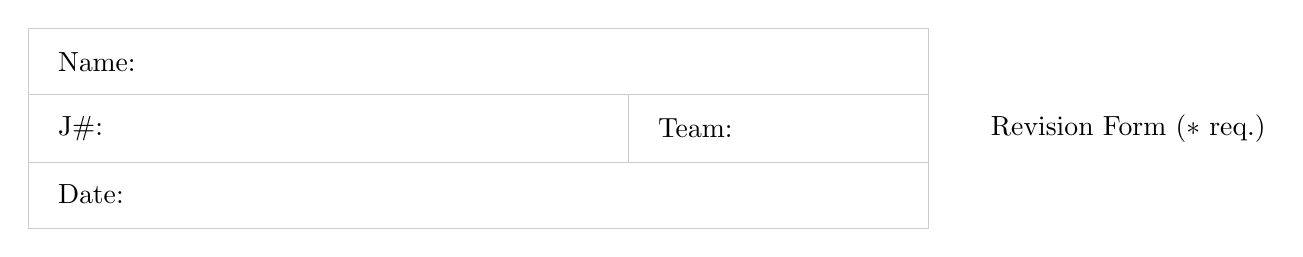
\begin{tikzpicture}[x=1in,y=1in]
  \draw[color=black!20] (0,0) rectangle (4.5,1);
  \draw[color=black!20] (0,0.67) -- (4.5,0.67);
  \draw[color=black!20] (3,0.33) -- (3,0.67);
  \draw[color=black!20] (0,0.33) -- (4.5,0.33);

  \node[anchor=west] at (0.1,0.83) {Name:};
  \node[anchor=west] at (0.1,0.5) {J\#:};
  \node[anchor=west] at (3.1,0.5) {Team:};
  \node[anchor=west] at (0.1,0.17) {Date:};

  \node at (5.5,0.5) {Revision Form (\(\ast\) req.)};
\end{tikzpicture}

\vspace{1em}

\begin{tikzpicture}[x=1in,y=1in]
  \draw[color=black!50] (0,0) rectangle (6.4,1);
  \draw[color=black!50] (1,0) -- (1,1);
  \draw[color=black!50] (3.2,0) -- (3.2,1);
  \draw[color=black!50] (5.4,0) -- (5.4,1);

  \node[anchor=north west,color=black!70] at (0,0.95) {\footnotesize Standard:};
  \node[anchor=north west,color=black!70] at (1,0.95) {\footnotesize Mastery Quiz:};
  \node[anchor=north west,color=black!70] at (3.2,0.95) {\footnotesize Exercise Version:};
  \node[anchor=north west,color=black!70] at (5.4,0.95) {\footnotesize New Mark:};
\end{tikzpicture}

Complete all fields at the top of the page (except ``New Mark''),
and use the provided space to write a \textbf{complete revised solution}
for an allowed revision.
You do not need to rewrite the question. 
It's highly recommended you complete this form in pencil. 

\vfill

This form is due promptly after a revision mark has been returned, usually
the following Tuesday. Late forms will not be accepted.

\(\square\) If this box is marked by the instructor, 
you may re-revise your solution one final time by editing
your solution on this sheet and resubmitting by the next class meeting. 
\end{document}
